% ============================================================
%  KrishokChat — Capstone Design & Innovation Challenge poster
%  A0 LANDSCAPE (118.9 x 84.1 cm) · 5 columns
%  Theme: gemini + custom "krishok" colours
%
%  >>> COMPILE WITH LUALATEX <<<   (MiKTeX fontconfig fix, 2026-08-19)
%
%  Content: POSTER_CONTENT_PLAN.md (approved)
%  Numbers: poster_stats.yaml (single source of truth)
% ============================================================

\documentclass[final]{beamer}

\usepackage[size=custom,width=118.9,height=84.1,scale=1.0]{beamerposter}
\usetheme{gemini}
\usecolortheme{krishok}

\usepackage{fontspec}
\usepackage{graphicx}
\usepackage{booktabs}
\usepackage{array}
\usepackage{tikz}
\usetikzlibrary{arrows.meta}
\usepackage{pgfplots}
\pgfplotsset{compat=1.18}
\usepackage{anyfontsize}
\usepackage{ragged2e}
\usepackage{qrcode}

% Body font: Regular weight for print legibility (theme loads Light)
\setsansfont{Lato}[
  Path=./fonts/,
  UprightFont=Lato-Regular.ttf,
  BoldFont=Lato-Bold.ttf,
  ItalicFont=Lato-Italic.ttf,
  BoldItalicFont=Lato-Bold.ttf
]

% ---------- Bengali ----------
\newfontfamily\bengalifont{Noto Serif Bengali}[
  Path=./fonts/,
  UprightFont=NotoSerifBengali-Regular.ttf,
  BoldFont=NotoSerifBengali-Bold.ttf,
  Script=Bengali
]
\newcommand{\bn}[1]{{\bengalifont #1}}

\graphicspath{{./img/}{./assets/}}

% extra chart colour (stays in the grey-green family)
\definecolor{barGrey}{HTML}{AEBBAF}

% ====================
% Column geometry — 5 columns
% (N+1)*sepwidth + N*colwidth = paperwidth
% 6(0.018) + 5(0.1784) = 0.108 + 0.892 = 1.000
% ====================
\newlength{\sepwidth}\setlength{\sepwidth}{0.018\paperwidth}
\newlength{\colwidth}\setlength{\colwidth}{0.1784\paperwidth}
\newlength{\ribbonwidth}\setlength{\ribbonwidth}{0.964\paperwidth}
\newcommand{\separatorcolumn}{\begin{column}{\sepwidth}\end{column}}

% ====================
% Compact headline
% ====================
\setbeamerfont{headline title}{size=\LARGE,series=\bfseries}
\setbeamerfont{headline author}{size=\large}
\setbeamerfont{headline institute}{size=\normalsize}
\setbeamerfont{block title}{size=\Large,series=\bfseries}

\setbeamertemplate{headline}{
  \begin{beamercolorbox}{headline}
    \vskip2ex
    \begin{columns}[c]
      \begin{column}{0.10\paperwidth}
        \centering
\includegraphics[height=6.5cm]{assets/NSU_Logo.png}
      \end{column}
      \begin{column}{0.82\paperwidth}
        \centering
        {\usebeamerfont{headline title}\usebeamercolor[fg]{headline title}\inserttitle\\[0.8ex]}
        {\usebeamerfont{headline author}\usebeamercolor[fg]{headline author}\insertauthor\\[0.6ex]}
        {\usebeamerfont{headline institute}\usebeamercolor[fg]{headline institute}\insertinstitute}
      \end{column}
      \begin{column}{0.08\paperwidth}
        \centering
        {\color{leaf}\fontsize{20}{24}\selectfont\bfseries CAPSTONE\\2026\\[1ex]\normalfont\vspace{-1ex}\fontsize{16}{20}\selectfont NSU \cdot ECE}
      \end{column}
    \end{columns}
    \vskip2ex
    \begin{beamercolorbox}[wd=\paperwidth,colsep=0.25ex]{headline rule}\end{beamercolorbox}
  \end{beamercolorbox}
}

% ====================
% Number macros — SINGLE SOURCE OF TRUTH (poster_stats.yaml)
% If a number is not defined here, it does not go on the poster.
% ====================
\newcommand{\Nbench}{85{,}979}
\newcommand{\Nnodes}{2{,}882}
\newcommand{\Npubs}{284}
\newcommand{\Ninst}{13}
\newcommand{\Ntriples}{17{,}501}
\newcommand{\Nentities}{19{,}768}
\newcommand{\Nfarmerq}{1{,}000}
\newcommand{\Ninterviews}{300}
\newcommand{\Ndialects}{6}
\newcommand{\Nsoil}{722}
\newcommand{\Nseries}{46}
\newcommand{\Ncrops}{14}
\newcommand{\RhybridRRF}{0.539}
\newcommand{\Rbm}{0.506}
\newcommand{\Rdense}{0.464}
\newcommand{\Rdensecolloq}{0.093}
\newcommand{\Rdenseformal}{0.970}
\newcommand{\Rbmcross}{0.004}
\newcommand{\Rcolbert}{0.487}
\newcommand{\Rbge}{0.408}
\newcommand{\FoneOurs}{0.314}
\newcommand{\FoneLlama}{0.165}
\newcommand{\FoneGemini}{0.104}
\newcommand{\FoneGemma}{0.087}
\newcommand{\Fonegain}{1.9$\times$}
\newcommand{\Pval}{$p\!\approx\!6.7\times10^{-5}$}
\newcommand{\AccBrassica}{97.29\%}
\newcommand{\AccCorn}{97.23\%}
\newcommand{\AccRice}{96.49\%}
\newcommand{\AccPotato}{95.04\%}
\newcommand{\AccWheat}{88.00\%}
\newcommand{\LibCoverage}{436/437}
\newcommand{\Households}{47 million}
\newcommand{\YieldLoss}{20--40\%}
\newcommand{\Ncalls}{92{,}094}
\newcommand{\Krishi}{16123}
\newcommand{\Emergency}{999}
\newcommand{\HallucFloor}{4.05--7.00\%}
\newcommand{\EntityGap}{92\%}
\newcommand{\NonCompliance}{0.31\%}
\newcommand{\Paisa}{2 paisa}
\newcommand{\GpuCost}{\$497}
\newcommand{\GpuCap}{13 million}
\newcommand{\SmartphoneOwn}{73.4\%}
\newcommand{\RuralNet}{43.6\%}
\newcommand{\FosholiUsers}{2.6M}
\newcommand{\WaterSave}{63\%}
\newcommand{\UreaSave}{50\%}

% ====================
% Components
% ====================
\newcommand{\figbox}[2]{%
  \begin{center}\setlength{\fboxrule}{1pt}\setlength{\fboxsep}{0pt}%
  {\color{rulegrey}\fbox{\parbox[c][#1][c]{\linewidth}{%
    \centering\color{leaf}\normalsize\textsc{#2}}}}\end{center}}

\newcommand{\yes}{{\color{leaf}\textbf{\Large$\bullet$}}}
\newcommand{\nomark}{{\color{rulegrey}\textbf{\Large--}}}
\newcommand{\partmark}{{\color{ochre}\textbf{\Large$\circ$}}}

\newcommand{\solobar}[1]{%
  \begin{tikzpicture}[baseline=0mm]\fill[leaf](0,0)rectangle({#1*3.0},0.30);\end{tikzpicture}}

\newcommand{\statchip}[3]{%
  \begin{minipage}[t]{\linewidth}\centering
    {\color{#1}\fontsize{40}{44}\selectfont\textbf{#2}}\\[0.3ex]
    {\color{ink}\small #3}\end{minipage}}

\newcommand{\badge}[2]{%
  \colorbox{white}{\parbox[c][2.0cm][c]{0.30\linewidth}{%
    \centering{\color{leaf}\large\textbf{#1}}\\{\footnotesize #2}}}}

% ====================
% Title
% ====================
\title{KrishokChat: A Safety-First Agentic Agricultural Advisory System for Bangladeshi Smallholder Farmers}
\author{Khan Raiyan Ibne Reza \and Sanjana Aktar Maria \and Shakil Ahmed}
\institute{Department of Electrical and Computer Engineering, North South University
  \samelineand Institute of Water and Flood Management, BUET
  \samelineand Advisor: Dr.~Sumaiya Tabassum Nimi}

\footercontent{
  {\footnotesize
  [1] KrishokChat: A Provenance-Traceable Multi-Task Bengali Agricultural Benchmark with Safety-Critical Chemical Advisory --- EACL 2026, under review \quad
  [2] AgriTrust --- SIGIR-AP 2026, under review \quad
  [3] AgriVision BD --- edge crop-disease classification report, 2026\\[0.5ex]
  \texttt{github.com/RaiyaanReza/KrishokChat-Agricultural-Advisory-System} \quad
  \texttt{huggingface.co/RaiyanKhaan/KrishokChat-Advisory-System} \quad
  {\color{clay}\textbf{Emergency triage: \Krishi{} / \Emergency}}}
}

% ============================================================
\begin{document}
\begin{frame}[t]

% ---------------- ROW 1: STAT RIBBON ----------------
\begin{columns}[t]
\separatorcolumn
\begin{column}{\ribbonwidth}
  \begin{columns}[t]
    \begin{column}{0.1633\textwidth}\statchip{leaf}{\Nbench}{benchmark instances, 4 tracks}\end{column}
    \begin{column}{0.1633\textwidth}\statchip{leaf}{\Fonegain}{Bengali QA over best zero-shot}\end{column}
    \begin{column}{0.1633\textwidth}\statchip{leaf}{95--97\%}{on-device crop diagnosis}\end{column}
    \begin{column}{0.1633\textwidth}\statchip{leaf}{$<$30 ms}{offline Android inference}\end{column}
    \begin{column}{0.1633\textwidth}\statchip{leaf}{\Paisa}{marginal cost per AI answer}\end{column}
    \begin{column}{0.1633\textwidth}\statchip{clay}{\Krishi}{human escalation, always free}\end{column}
  \end{columns}
  \vspace{0.5ex}{\color{rulegrey}\rule{\linewidth}{2pt}}\vspace{0.5ex}
\end{column}
\separatorcolumn
\end{columns}

% ---------------- ROW 2: FIVE COLUMNS ----------------
\begin{columns}[t]
\separatorcolumn

% ========== COLUMN 1 — WHY: PROBLEM, IDEA, IMPACT ==========
\begin{column}{\colwidth}

  \begin{block}{The Problem}
    Bangladesh's \Households{} farming households have no reliable advisory in their
    own language. Undetected crop disease costs \YieldLoss{} of yield. A wrong
    pesticide dose can poison a family and contaminate the water supply --- and a
    generic chatbot, asked for a dosage, will always answer, right or wrong.
  \end{block}

  \begin{block}{The Idea: An Evidence-Grounded Trust Stack}
    Not a chatbot with an agriculture prompt. A layered trust stack, built on our own
    research: official publications $\rightarrow$ machine-readable knowledge graph
    $\rightarrow$ provenance-verified retrieval $\rightarrow$ a safety gate
    \textbf{before} the model ever runs $\rightarrow$ dosage verification $\rightarrow$
    an answer with citations, or human escalation.

    Every layer exists because our measurements showed it must (column 4).
  \end{block}

  \begin{block}{Impact: Safety, Environment, Access}
    \textbf{Health.} Unsafe agrochemical queries are refused and escalated --- to the
    \Krishi{} Krishi Call Center and \Emergency{} --- in every tier of the product.
    Safety is never paywalled.

    \textbf{Environment.} Source-verified dosing cuts over-application of pesticide
    and fertiliser. Independent Bangladesh sensor-irrigation trials report up to
    \WaterSave{} water and \UreaSave{} urea savings --- the direction our soil-vision
    lane targets.

    \textbf{Access.} Runs in Bengali --- standard and dialect --- with voice input,
    offline on the mid-range Android phones farmers already own.
  \end{block}

  \begin{block}{What Exists vs What We Added}
    \begin{tabular}{@{}p{0.52\linewidth}ccc@{}}
      \toprule
      \textbf{Capability} & \textbf{Generic} & \textbf{K.B.} & \textbf{Ours} \\ \midrule
      Safety check before retrieval        & \nomark   & \nomark   & \yes \\
      14-field dosage verifier             & \nomark   & \nomark   & \yes \\
      Audit log + analytics panel          & \nomark   & \nomark   & \yes \\
      Bengali + \Ndialects{} dialects      & \partmark & \partmark & \yes \\
      Published \Nbench{} benchmark        & \nomark   & \partmark & \yes \\
      Photo $\rightarrow$ grounded treatment & \partmark & \nomark & \yes \\
      Field soil dataset                   & \nomark   & \nomark   & \yes \\
      \bottomrule
    \end{tabular}

    \vspace{0.5ex}
    {\footnotesize \yes\ present \quad \partmark\ partial \quad \nomark\ absent
    \quad K.B.\ = KrishokBondhu}
  \end{block}

  \begin{exampleblock}{Ongoing \& Next}
    Voice output for low-literacy users $\cdot$ extended dialect coverage $\cdot$
    soil-vision refinement toward irrigation advisories $\cdot$ district-level pilot
    with an extension office.
  \end{exampleblock}

\end{column}

\separatorcolumn

% ========== COLUMN 2 — WHAT WE BUILT (research) ==========
\begin{column}{\colwidth}

  \begin{block}{The Foundation: Four Research Assets}
    {\small
    \begin{tabular}{@{}p{0.21\linewidth}p{0.27\linewidth}p{0.47\linewidth}@{}}
      \toprule
      \textbf{Asset} & \textbf{Scale} & \textbf{Ground truth \& provenance} \\ \midrule
      Benchmark, 4 tracks & \Nbench{} instances &
        General QA 28{,}993 · Treatment 11{,}224 (66.3\% chemical-bearing) ·
        Table 25{,}650 · Safety 20{,}112 --- every instance citation-traced \\
      Knowledge graph & \Nnodes{} nodes · \Ntriples{} triples &
        \Nentities{} entities extracted from \Npubs{} publications · \Ninst{}
        institutions (BARC, BARI, BRRI, DAE, \ldots) \\
      Farmer-language benchmark & \Nfarmerq{} queries &
        \Ninterviews{} face-to-face interviews (Rajshahi \& Natore) + farmer
        groups · \Ndialects{} dialects \\
      Soil-moisture dataset & \Nsoil{} field RGB images &
        paired tensiometer readings 0.0--21.5 kPa · 6 USDA textures · \Ncrops{}
        crops · \Nseries{} leakage-checked series · Pabna, May 2026 \\
      \bottomrule
    \end{tabular}}

    \vspace{0.5ex}
    {\footnotesize All released CC-BY-4.0 on Hugging Face.}
  \end{block}

  \begin{block}{Grounded in Bangladesh}
    \begin{center}
      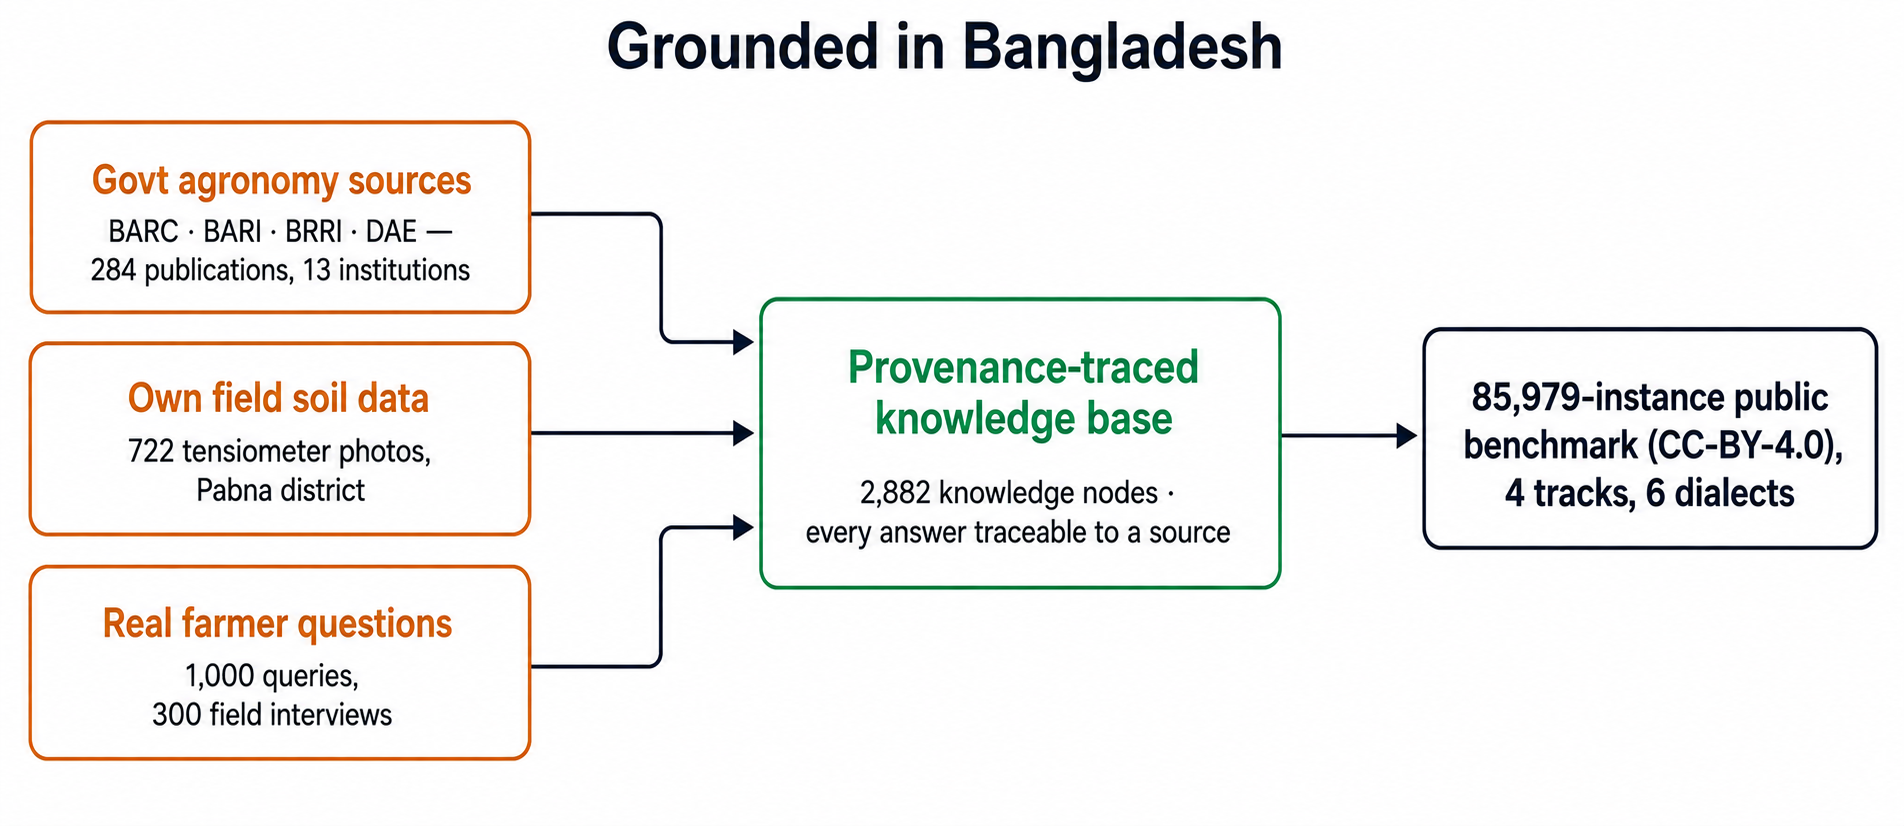
\includegraphics[width=\linewidth]{D3_grounded_data.png}
    \end{center}
    {\footnotesize From official publications to provenance-traced retrieval nodes.}
  \end{block}

  \begin{block}{Built From the Field, Not the Web}
    \begin{center}
      \begin{tabular}{@{}c@{\hspace{0.4cm}}c@{\hspace{0.4cm}}c@{}}
        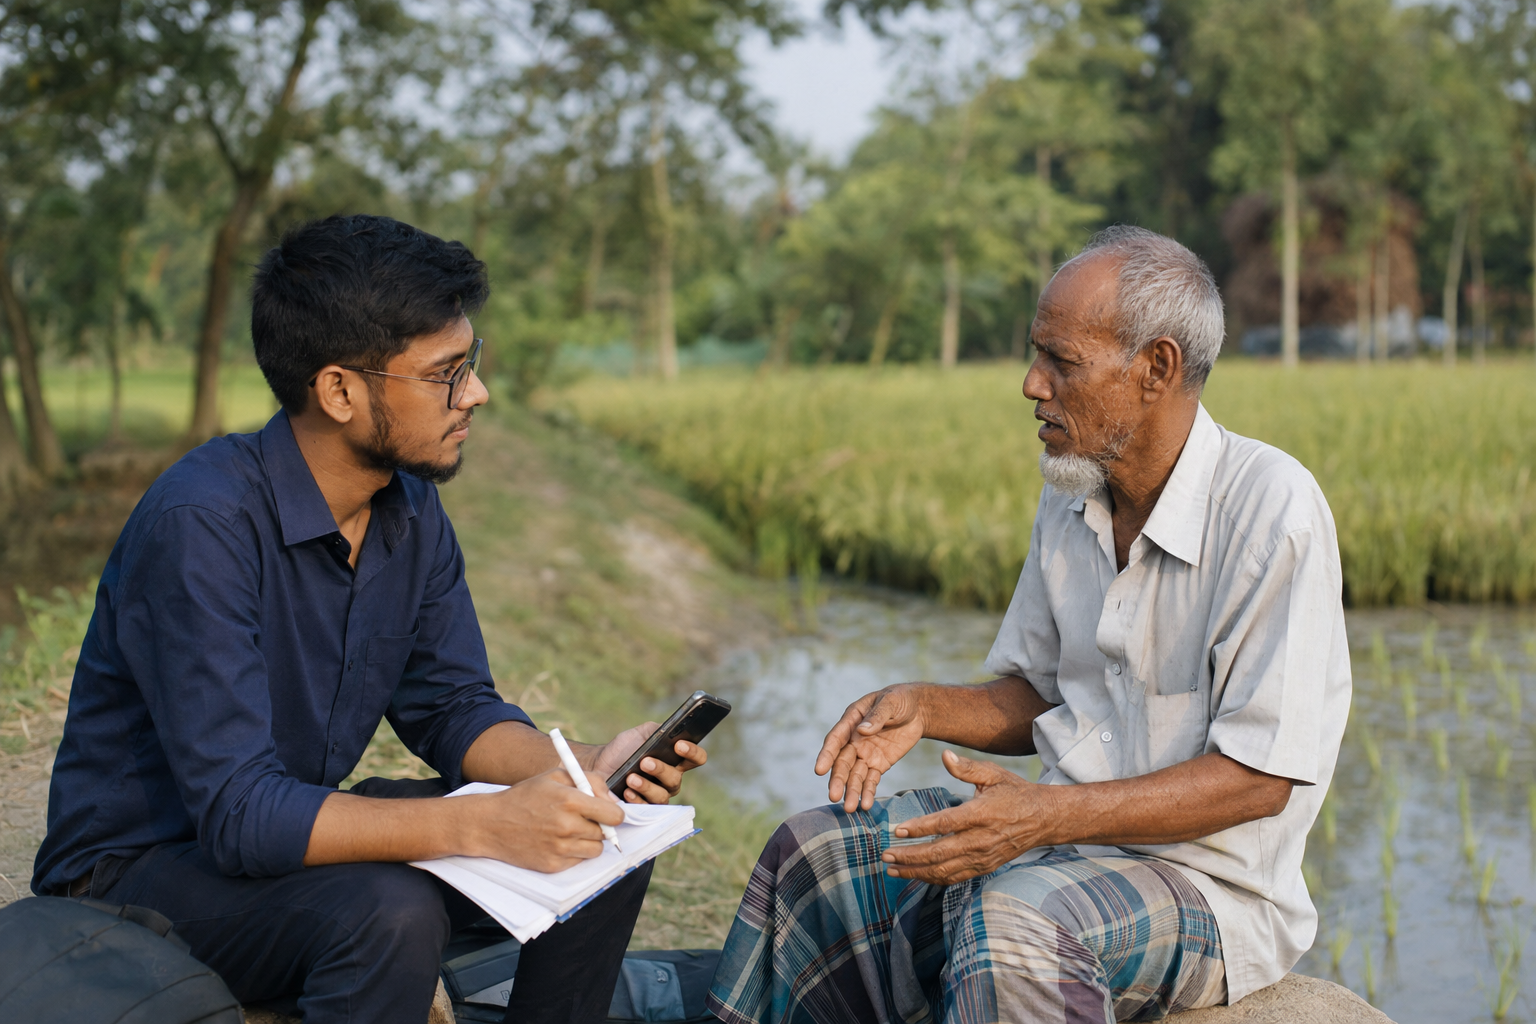
\includegraphics[height=5.6cm]{researcher_interviewing_farmer.png} &
        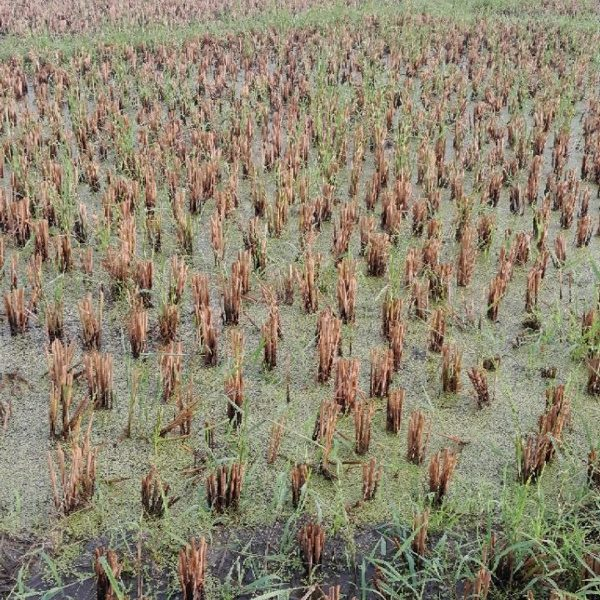
\includegraphics[height=4.1cm]{soil_wet.jpg} &
        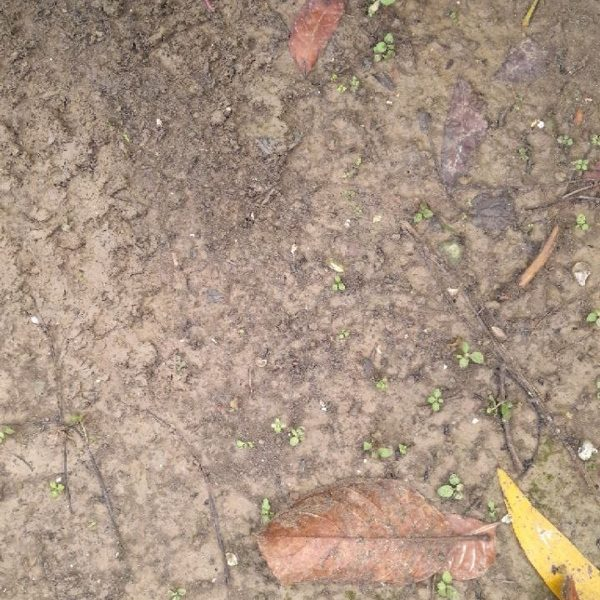
\includegraphics[height=4.1cm]{soil_dry.jpg} \\[-0.5ex]
        {\scriptsize 300 farmer interviews} &
        {\scriptsize 0.0 kPa (wet)} &
        {\scriptsize 8.0 kPa (dry)} \\
      \end{tabular}
    \end{center}
    \vspace{0.5ex}
    {\small
    \begin{itemize}
      \item \textbf{Page-level provenance} --- every answer traceable to a publication and page.
      \item \textbf{Physical ground truth} --- tensiometer kPa readings, not annotator opinion.
      \item \textbf{Series-stratified splits} --- no near-duplicate leakage between train and test.
    \end{itemize}}
  \end{block}

\end{column}

\separatorcolumn

% ========== COLUMN 3 — MEASURED RESULTS (proof) ==========
\begin{column}{\colwidth}

  \begin{alertblock}{Our On-Device Model Beats Far Larger Ones}
    \begin{center}
    \begin{tikzpicture}
      \begin{axis}[
        width=\linewidth, height=9.6cm,
        xbar, xmin=0, xmax=0.36,
        y axis line style={draw=none},
        axis x line*=bottom,
        tick style={draw=none},
        ytick=data,
        yticklabels={Gemma-4-26B, Gemini-2.5-Flash-Lite, LLaMA-3.1-8B, KrishokChat-4B (ours)},
        yticklabel style={font=\small},
        xticklabel style={font=\small},
        xlabel={\small Token-F1, Bengali general QA},
        every node near coord/.append style={font=\small\bfseries,color=ink},
        nodes near coords,
        nodes near coords align={horizontal},
        enlarge y limits=0.28,
        y=11mm,
        bar width=7mm,
      ]
        \addplot[fill=barGrey] coordinates {(0.087,0) (0.104,1) (0.165,2)};
        \addplot[fill=leaf] coordinates {(0.314,3)};
      \end{axis}
    \end{tikzpicture}
    \end{center}
    \vspace{-1ex}
    {\small \textbf{\Fonegain{} the best zero-shot baseline} (\Pval). LoRA fine-tune of
    Gemma-4-E4B, 4-bit quantised --- deployable on-device.}
  \end{alertblock}

  \begin{alertblock}{Retrieval: Hybrid Beats Every Single Method}
    \begin{center}
    \begin{tikzpicture}
      \begin{axis}[
        width=\linewidth, height=7.4cm,
        xbar, xmin=0, xmax=0.62,
        y axis line style={draw=none},
        axis x line*=bottom,
        tick style={draw=none},
        ytick=data,
        yticklabels={BGE-M3, Dense, ColBERT, BM25, Hybrid RRF (ours)},
        yticklabel style={font=\small},
        xticklabel style={font=\small},
        xlabel={\small Recall@10, 900 answerable farmer queries},
        every node near coord/.append style={font=\small\bfseries,color=ink},
        nodes near coords,
        enlarge y limits=0.3,
        y=10mm,
        bar width=5.5mm,
      ]
        \addplot[fill=barGrey] coordinates {(0.408,0) (0.464,1) (0.487,2) (0.506,3)};
        \addplot[fill=leaf] coordinates {(0.539,4)};
      \end{axis}
    \end{tikzpicture}
    \end{center}
    \vspace{-1ex}
    {\small +9\% over dense retrieval ($p<0.001$, Wilcoxon).}
  \end{alertblock}

  \begin{alertblock}{Crop Disease, On-Device}
    \vspace{-0.5ex}
    {\small
    \begin{tabular}{@{}lrl@{}}
      Brassica (11 classes) & \AccBrassica & \solobar{1.00} \\
      Corn (4 classes)      & \AccCorn     & \solobar{1.00} \\
      Rice (8 classes)      & \AccRice     & \solobar{0.99} \\
      Potato (3 classes)    & \AccPotato   & \solobar{0.97} \\
      Wheat (live sweep)    & \AccWheat    & \solobar{0.90} \\
    \end{tabular}}

    \vspace{0.5ex}
    \noindent\begin{tabular}{@{}c@{\hspace{0.15cm}}c@{}}
      \badge{\LibCoverage}{grounded Bengali treatment (99.8\%)} &
      \badge{$<$30 ms}{on-device, Android} \\
    \end{tabular}
  \end{alertblock}

  \begin{alertblock}{Safety Behaviour}
    {\small 1 of 323 unsafe test queries leaked through --- \NonCompliance{}
    non-compliance. Fail-closed by design: missing evidence means abstain.}
  \end{alertblock}

  {\scriptsize Test sets: benchmark held-out split · 900 answerable queries ·
  per-crop held-out images. Disease = classification top-1.}

\end{column}

\separatorcolumn

% ========== COLUMN 4 — FINDINGS → ARCHITECTURE (application) ==========
\begin{column}{\colwidth}

  \begin{block}{Four Measured Failures $\rightarrow$ Four Design Decisions}
    {\small
    \begin{tabular}{@{}p{0.47\linewidth}p{0.49\linewidth}@{}}
      \toprule
      \textbf{Measured failure} & \textbf{Our design answer} \\ \midrule
      LLMs hallucinate chemical dosages at \HallucFloor{} even with gold evidence
        & Safety gate \textbf{before} retrieval + 14-field fail-closed verifier \\
      Dense retrieval collapses on farmer language: R@10 \Rdenseformal{} formal
        $\rightarrow$ \Rdensecolloq{} colloquial
        & Hybrid BM25 + dense, RRF fusion \\
      \EntityGap{} of formal entities never appear in farmer queries ---
        \bn{পাতা হলুদ হয়ে যাচ্ছে} $\neq$ ``Yellow Mosaic Virus''
        & Register-aware retrieval across \Ndialects{} dialects \\
      The national helpline answered \Ncalls{} calls last year
        & AI triage: auto-answer routine, escalate high-risk to humans \\
      \bottomrule
    \end{tabular}}
  \end{block}

  \begin{block}{System Architecture}
    \begin{center}
    \begin{tikzpicture}[
        stage/.style={rectangle, rounded corners=4pt, fill=leaf, text=white,
          text width=10.2cm, align=center, minimum height=1.55cm, font=\small\bfseries},
        query/.style={rectangle, rounded corners=4pt, draw=leaf, thick, fill=leaflight,
          text width=10.2cm, align=center, minimum height=1.2cm, font=\small\bfseries},
        result/.style={rectangle, rounded corners=4pt, fill=leaf!85!black, text=white,
          text width=10.2cm, align=center, minimum height=1.45cm, font=\small\bfseries},
        exitbox/.style={rectangle, rounded corners=4pt, draw=clay, very thick,
          fill=white, text=clay, text width=6.4cm, align=center,
          minimum height=2.3cm, font=\small\bfseries},
        audit/.style={rectangle, rounded corners=4pt, draw=leaf, dashed, thick,
          fill=papertint, text=ink, text width=6.4cm, align=center,
          minimum height=1.9cm, font=\small\bfseries},
        flow/.style={-{Stealth[length=3mm]}, leaf, very thick},
        stopflow/.style={-{Stealth[length=3mm]}, clay, very thick},
        dashflow/.style={-{Stealth[length=3mm]}, leaf, thick, dashed},
      ]
      % main pipeline (centered column)
      \node[query] (q) at (0,0)
        {FARMER QUERY\\{\footnotesize\mdseries Bengali, any dialect, text or voice}};
      \node[stage] (s1) at (0,-2.1)
        {1~SAFETY / ROUTER\\{\footnotesize\mdseries 6 categories · fail-closed}};
      \node[stage] (s2) at (0,-4.4)
        {2~HYBRID RETRIEVAL\\{\footnotesize\mdseries BM25 + dense · RRF fusion · top-5}};
      \node[stage] (s3) at (0,-6.7)
        {3~GENERATION\\{\footnotesize\mdseries KrishokChat-4B · 4-bit · streamed Bengali}};
      \node[stage] (s4) at (0,-9.0)
        {4~VERIFIER\\{\footnotesize\mdseries 14 fields · 6 relations · fail-closed}};
      \node[result] (a) at (0,-11.2)
        {GROUNDED BENGALI ANSWER\\{\footnotesize\mdseries with citations to source pages}};
      % red exit branch
      \node[exitbox] (stop) at (8.6,-3.2)
        {STOP\\[0.3ex]{\footnotesize\mdseries banned chemical\\ self-harm risk\\
        prompt injection\\[0.5ex]
        $\rightarrow$ \Krishi{} Krishi Call Center\\ $\rightarrow$ \Emergency{} emergency}};
      % audit rail
      \node[audit] (log) at (8.6,-8.6)
        {EVERY DECISION\\{\footnotesize\mdseries logged, local only}\\[0.3ex]
        {\small AUDIT LOG $\rightarrow$ /ANALYTICS}};
      % arrows
      \draw[flow] (q) -- (s1);
      \draw[flow] (s1) -- (s2);
      \draw[flow] (s2) -- (s3);
      \draw[flow] (s3) -- (s4);
      \draw[flow] (s4) -- (a);
      \draw[stopflow] (s1.east) -- node[above, font=\footnotesize\bfseries,
        text=clay]{unsafe} (stop.west);
      \draw[dashflow] (s4.east) -- (log.west);
    \end{tikzpicture}
    \end{center}
    \vspace{-1ex}
    {\footnotesize Unsafe categories stop at stage 1 --- retrieval, generation and
    verification never run.}
  \end{block}

  \begin{block}{Vision: Classify, Then Route}
    \begin{center}
      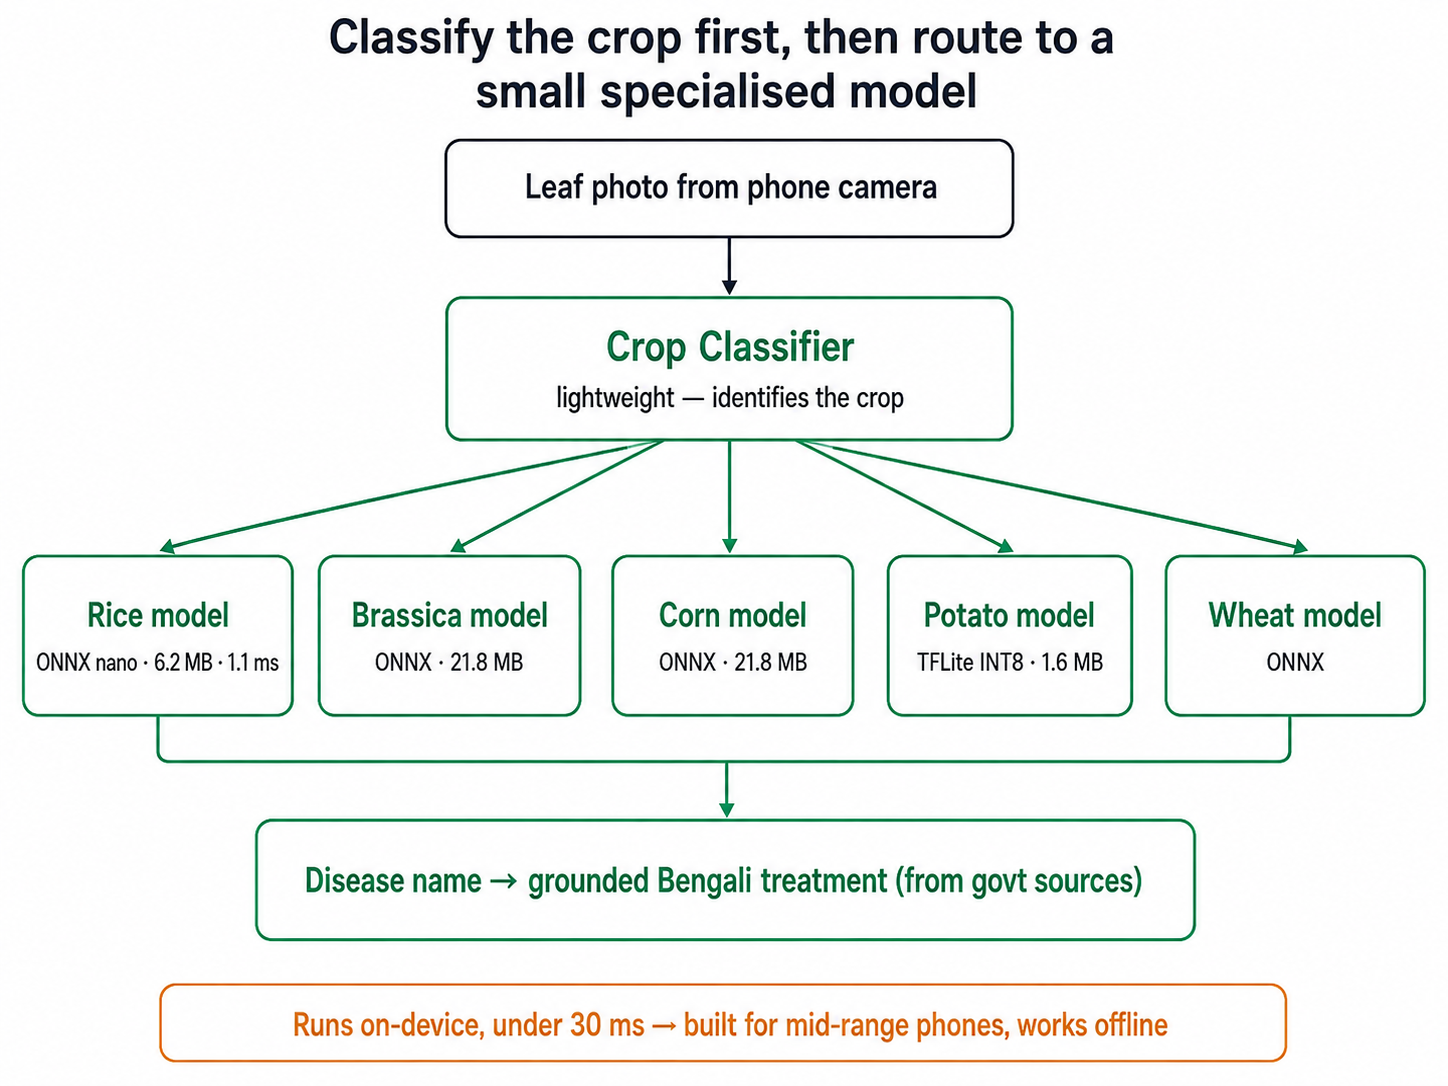
\includegraphics[width=\linewidth]{D2_disease_vision_routing.png}
    \end{center}
    {\footnotesize One photo $\rightarrow$ crop router $\rightarrow$ a small per-crop
    classifier $\rightarrow$ grounded Bengali treatment. The whole vision stack ships
    inside the app --- no server, no network needed.}
  \end{block}

\end{column}

\separatorcolumn

% ========== COLUMN 5 — PRODUCT · MARKET · MODEL ==========
\begin{column}{\colwidth}

  \begin{block}{The Product --- Krishi Patrak (\bn{কৃষি পত্রক})}
    \begin{center}
      \begin{tabular}{@{}c@{\hspace{0.35cm}}c@{\hspace{0.35cm}}c@{}}
        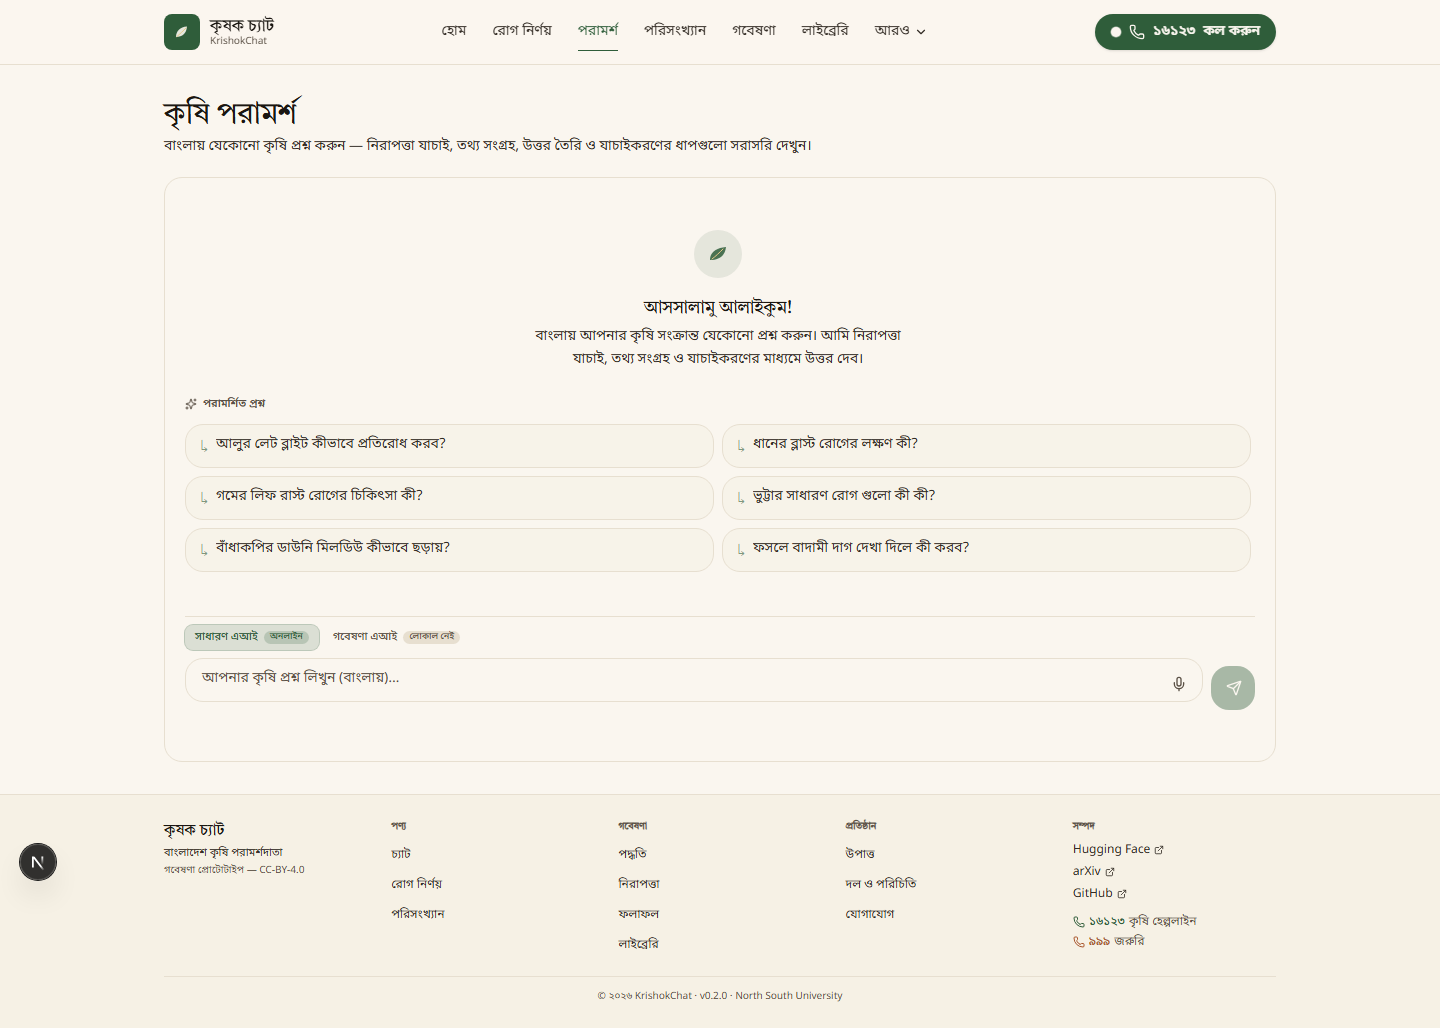
\includegraphics[width=0.27\linewidth]{shot_chat.png} &
        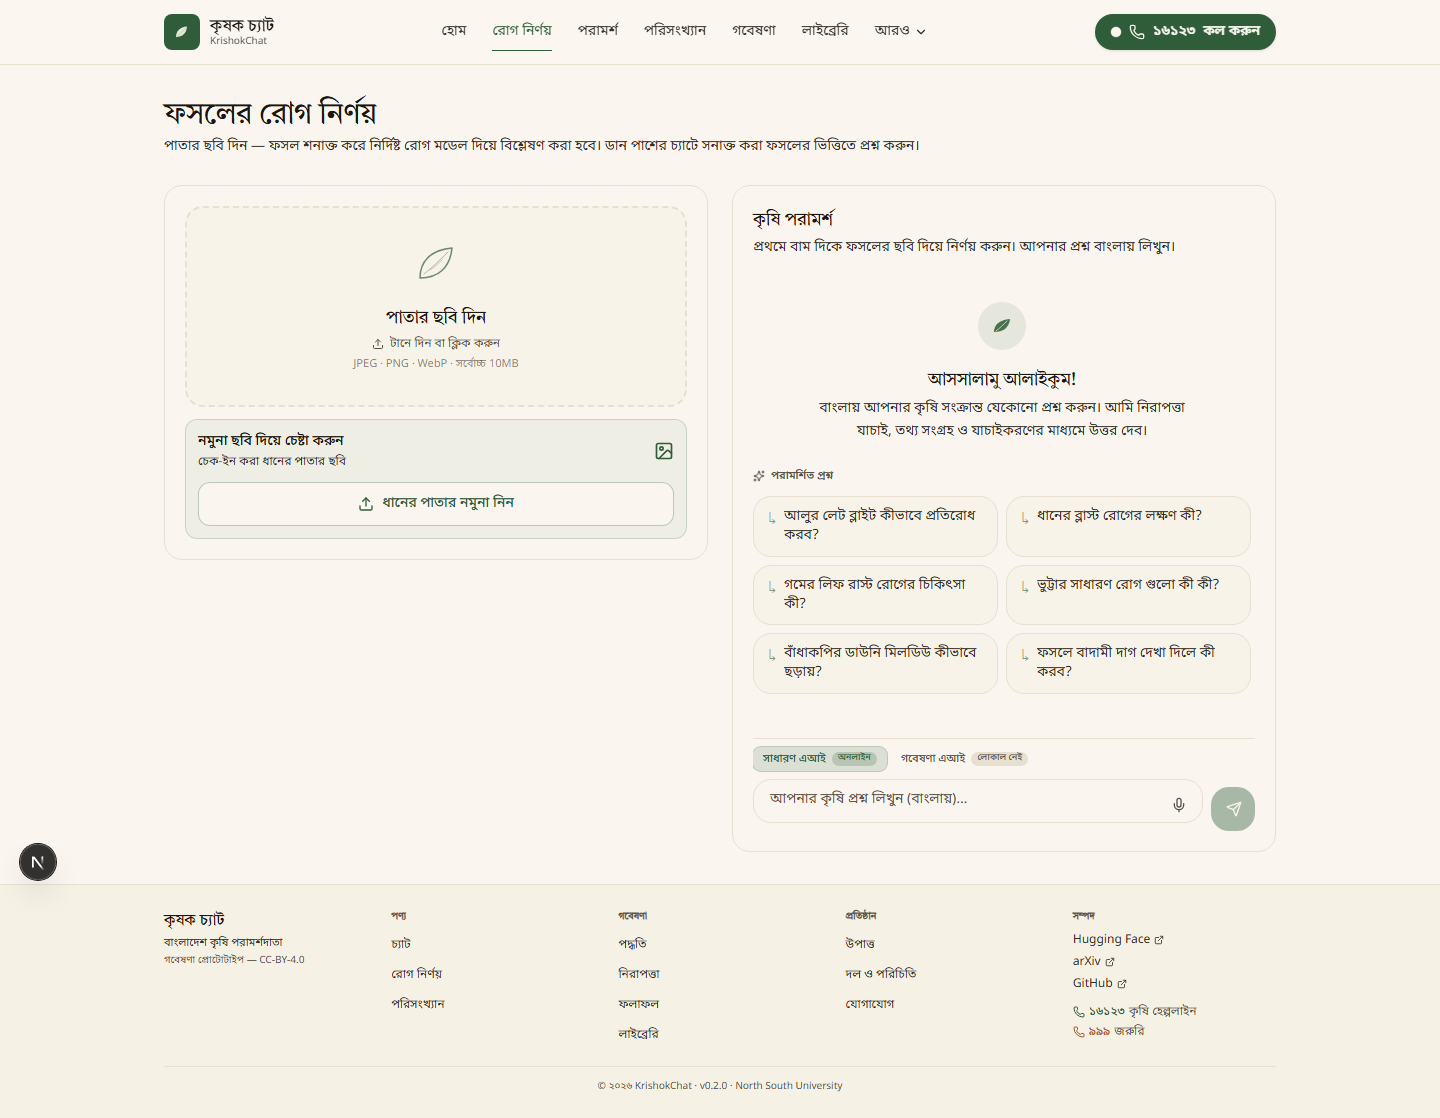
\includegraphics[width=0.27\linewidth]{shot_detect.png} &
        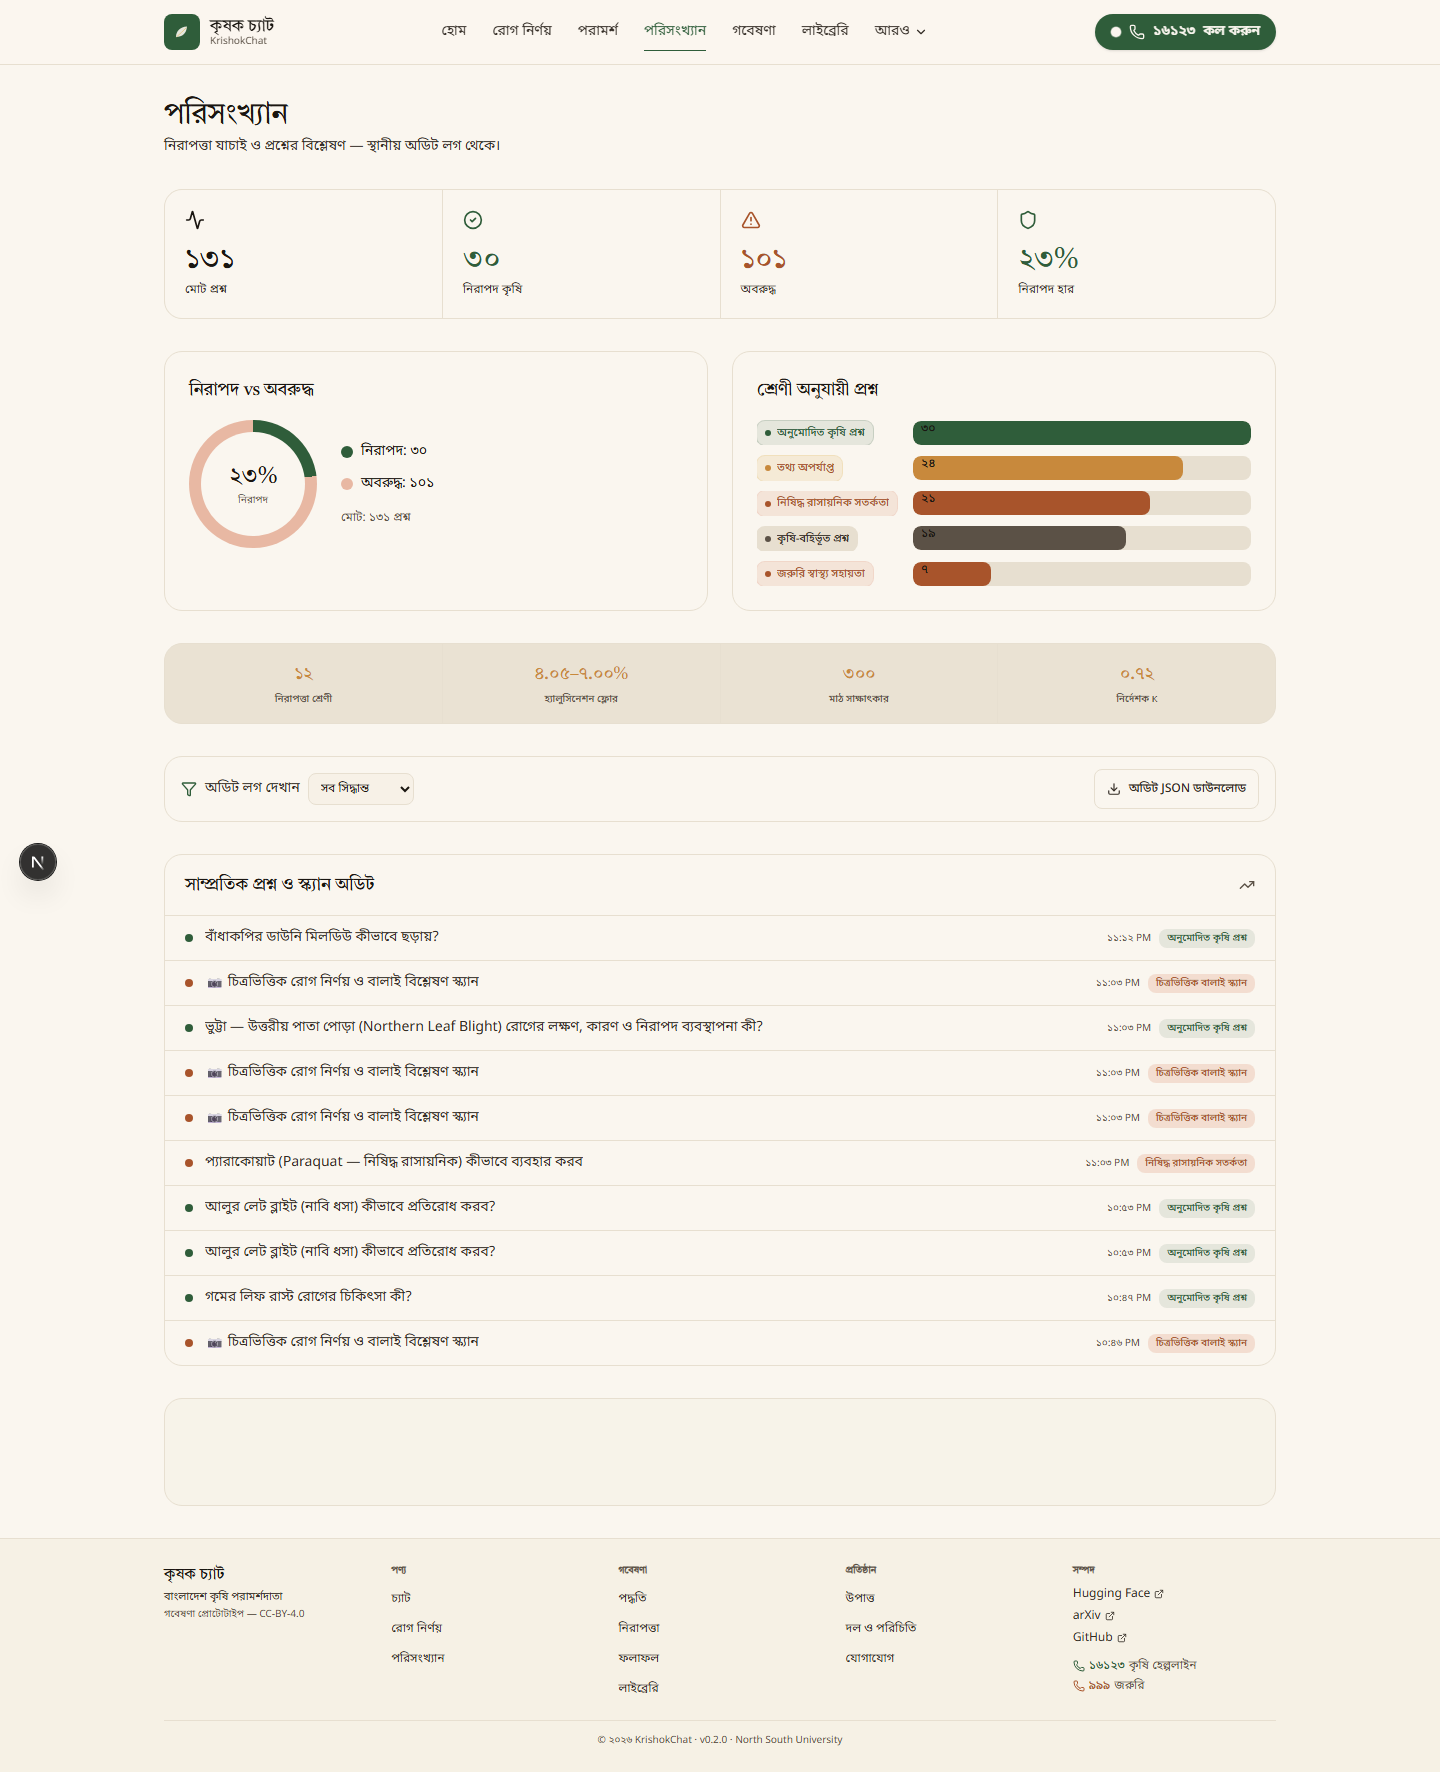
\includegraphics[width=0.27\linewidth]{shot_analytics.png} \\[-0.6ex]
        {\scriptsize Safety refusal $\rightarrow$ \Krishi} &
        {\scriptsize Photo $\rightarrow$ diagnosis} &
        {\scriptsize Audit dashboard} \\
      \end{tabular}
    \end{center}
    \vspace{0.5ex}
    {\small Bengali-first web + Android: live agent trace on every query, voice input,
    sunlight mode, offline-capable.}
  \end{block}

  \begin{block}{Market Readiness}
    {\small
    \textbf{What ships today.} Full-stack web app and Android app · on-device disease
    models that run with no network · live safety pipeline with audit dashboard ·
    437-entry treatment library verified end-to-end in live testing.

    \textbf{Why offline-first wins this market.} \SmartphoneOwn{} of households own a
    smartphone, but only \RuralNet{} of rural residents use the internet. An advisory
    app that needs the network loses half its users on arrival.

    \textbf{Scaling path.} Launch on a hosted API ($\approx$\Paisa{} per answer); at
    volume, one rented GPU ($\approx$\GpuCost{}/month) serves $\approx$\GpuCap{}
    answers monthly.}
  \end{block}

  \begin{exampleblock}{Business Model: Free for Farmers, Paid by Institutions}
    \figbox{11.0cm}{FREE vs PREMIUM tier diagram (GPT-generated, 4:3)\\[1ex]
      FREE: mapped answers from the grounded KB (no LLM --- cannot hallucinate)\\
      \quad + on-device photo diagnosis + safety gate + offline\\
      PREMIUM: everything in Free + open-ended conversation on our fine-tuned\\
      \quad model + priority + voice\\[0.5ex]
      banner: safety gate and \Krishi{} escalation identical in both tiers}

    \vspace{0.5ex}
    {\small
    \textbf{B2G.} AI triage front-end for the Krishi Call Center --- routine questions
    answered automatically, high-risk cases escalated with a full audit trail. The
    audit log is the trust asset for DAE / a2i.

    \textbf{B2B.} Analytics dashboard for agro-dealers, seed companies and NGOs:
    district-level insight into what farmers ask and which diseases surge. (ACI's
    Fosholi monetises its \FosholiUsers{} users the same way.)

    \textbf{Licensing.} The \Nbench-instance benchmark and \Nsoil-image soil dataset
    --- CC-BY-4.0 for research, commercial licence for agri-fintech and insurers.}
  \end{exampleblock}

  \begin{block}{Papers, Code \& Data}
    \begin{center}
    \begin{tabular}{@{}c@{\hspace{0.8cm}}c@{}}
      \qrcode[height=2.8cm]{https://huggingface.co/RaiyanKhaan/KrishokChat-Advisory-System} &
      \qrcode[height=2.8cm]{https://github.com/RaiyaanReza/KrishokChat-Agricultural-Advisory-System} \\[-0.5ex]
      {\scriptsize Dataset (Hugging Face)} & {\scriptsize Code (GitHub)} \\
    \end{tabular}
    \end{center}
    \vspace{0.3ex}
    {\scriptsize Full references in the footer.}
  \end{block}

\end{column}

\separatorcolumn
\end{columns}
\end{frame}
\end{document}
